% what the research has uncovered and to include most pertinent figures as evidence

\chapter{Results}
	
	% introduction: look back at conclusion from previous chapter; forward to contents of this chapter
	This chapter reports the graph measures obtained from the connectivity graphs, results of the statistical analysis and performances of trained classifiers.  
	

	\section{Graph Measures}
		
		Figure~\ref{fig:graphmeasure-witherror} shows the mean graph measure values for each band of interest, for each class. The same plot without the error bars can be seen in Fig.~\ref{fig:graphmeasure-noerror} in Appendix~\ref{appendix:extra-figures}. 
		
		% graph curve picture
		% graph measures with no error bars
		\begin{figure}
		    \centering
		    \captionsetup{justification=centering}
		    \begin{adjustwidth}{-5em}{-2em}
		    \centering
		    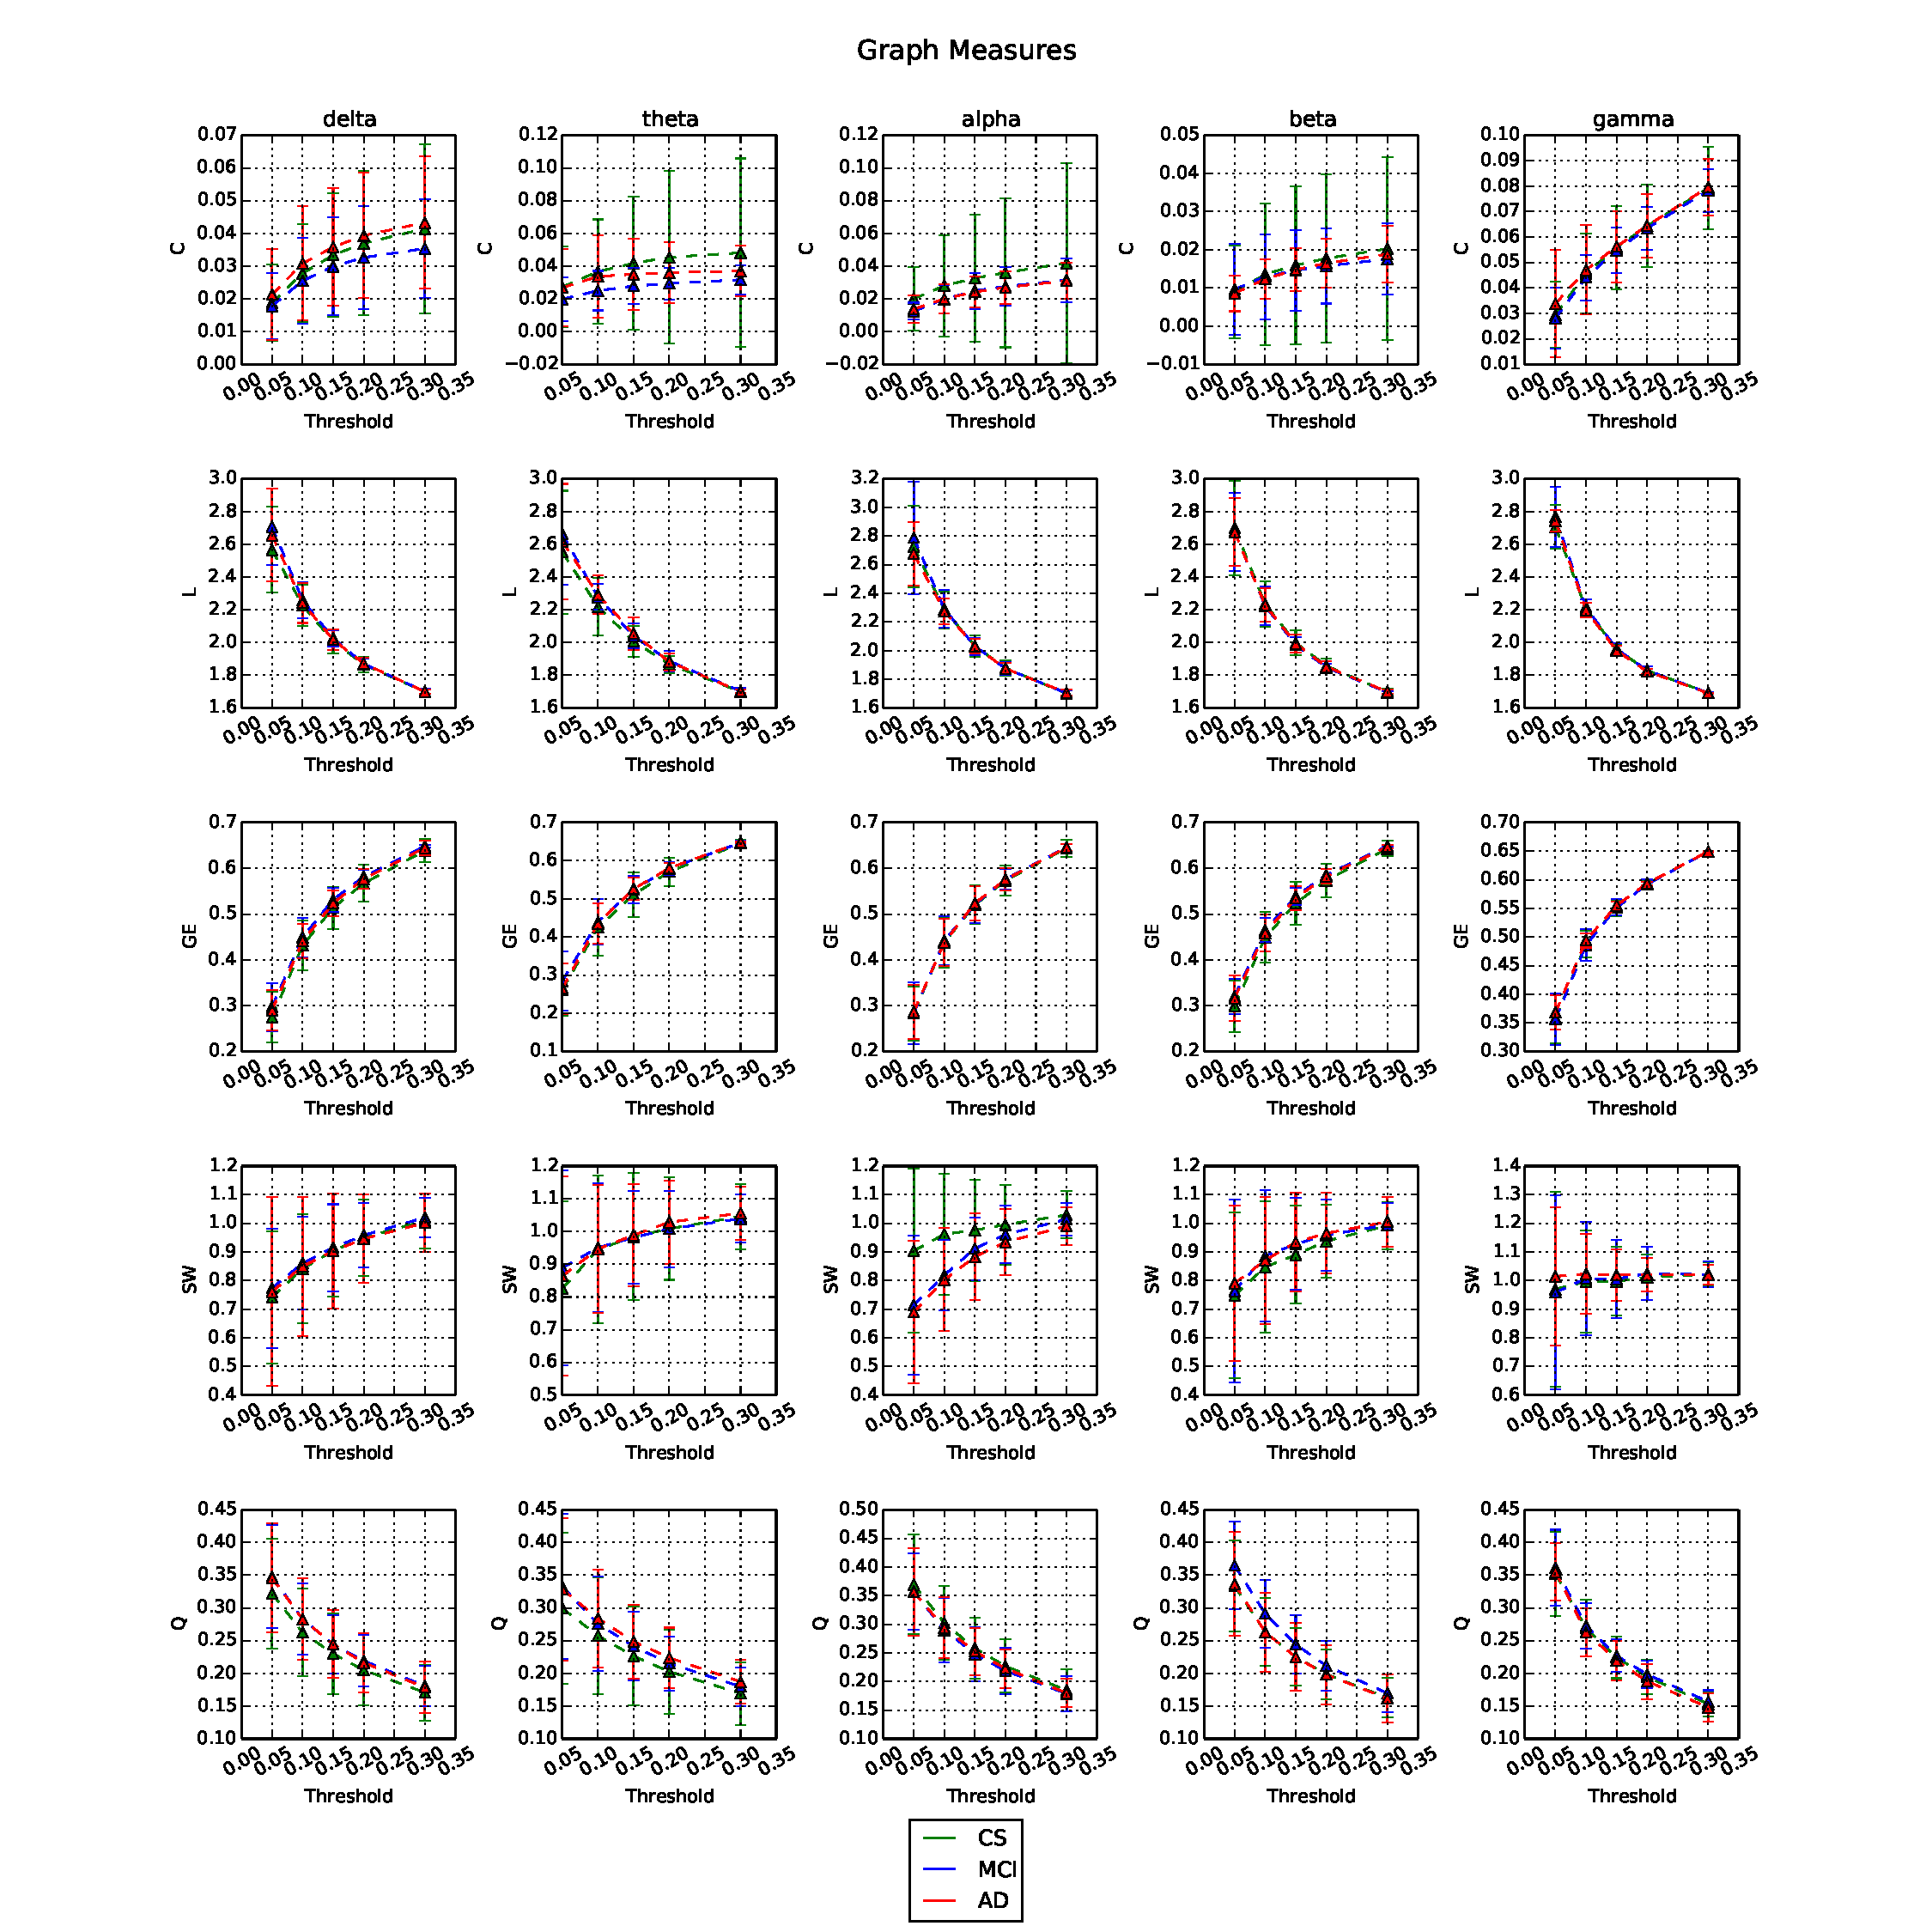
\includegraphics[scale=0.45]{GraphMeasuresWithErrorBar}
		    \end{adjustwidth}
		    \caption{Graph measures illustrating mean graph metric curves. Rows represent measures, columns represent frequency bands of interest. For each subplot, the \(x\) axis represents the threshold value and the \(y\) axis represents the graph measure value. C is the average clustering coefficient, L is the characteristic path length, GE is global efficiency, SW is the small-world measure and Q is modularity.}
		    \label{fig:graphmeasure-witherror}
		\end{figure}

	\section{Statistical Testing}
		\subsection{Functional Data Analysis}
		Statistical analysis using \ac{FDA} was performed between each pair of classes, for each graph metric and frequency band of interest. The top 20 most significant results (ordered by p-value) are showed in Table~\ref{tab:fda-top}. The full results of the \ac{FDA} statistical analysis can be found in Appendix~\ref{appendix:fda-full}. 

			\begin{table}
				\centering
				\begin{tabular}{|l|l|l|l|l|} \hline
					\textbf{Measure} & \textbf{Group A} & \textbf{Group B} & \textbf{Band} & \textbf{p-value} \\ \hline
					SW & CS  & AD  & alpha & 0.006  \\ 
					SW & CS  & MCI & alpha & 0.0657 \\
					GE & CS  & MCI & delta & 0.161  \\
					L  & CS  & MCI & delta & 0.1637 \\
					Q  & CS  & MCI & beta  & 0.1688 \\
					L  & CS  & AD  & gamma & 0.1691 \\
					GE & CS  & MCI & beta  & 0.1868 \\
					L  & CS  & AD  & theta & 0.1902 \\
					Q  & MCI & AD  & beta  & 0.1907 \\
					Q  & CS  & AD  & theta & 0.1912 \\
					C  & MCI & AD  & theta & 0.1914 \\
					C  & CS  & MCI & theta & 0.1942 \\
					GE & CS  & AD  & gamma & 0.2103 \\
					C  & MCI & AD  & delta & 0.2203 \\
					GE & MCI & AD  & gamma & 0.2224 \\
					L  & CS  & MCI & theta & 0.226  \\
					C  & CS  & AD  & alpha & 0.2401 \\
					GE & CS  & AD  & beta  & 0.2445 \\
					GE & CS  & AD  & delta & 0.252  \\
					Q  & CS  & AD  & delta & 0.2991 \\
				\hline
		    	\end{tabular}
			   	\caption{Results of the FDA statistics. Top 20 lowest p-values are listed. (see Appendix~\ref{appendix:fda-full} for full list.)}
			    \label{tab:fda-top}
			\end{table}

	\section{Data Visualisation}
		\subsection{t-SNE}
		
		The extracted graph features for each threshold were plotted using \ac{t-SNE} \autocite{Maaten2008}. Figures~\ref{fig:tsneT1} to \ref{fig:tsneT5} show the plots for each threshold. It can be seen that the datapoints of the \ac{AD}, \ac{MCI} and \ac{CS} classes are mixed and no particular clusters can be discerned. This suggests that the data would be hard to separate.

		% t-SNE plots
		\begin{figure}
			\centering
		    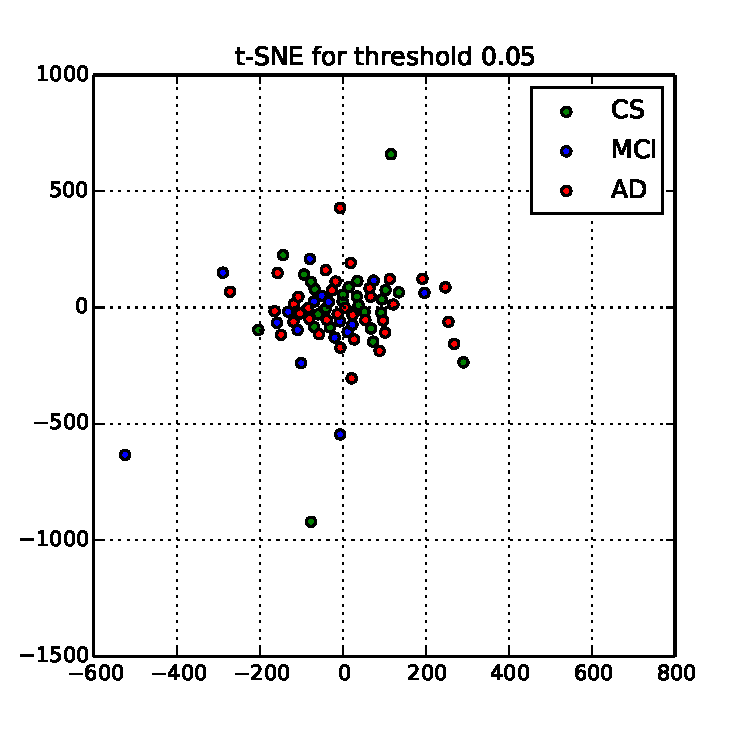
\includegraphics[width=0.7\textwidth]{tSNEThresh1}
		    \caption{t-SNE plot for threshold 0.05.}
		    \label{fig:tsneT1}
		\end{figure}
		\begin{figure}
			\centering
		    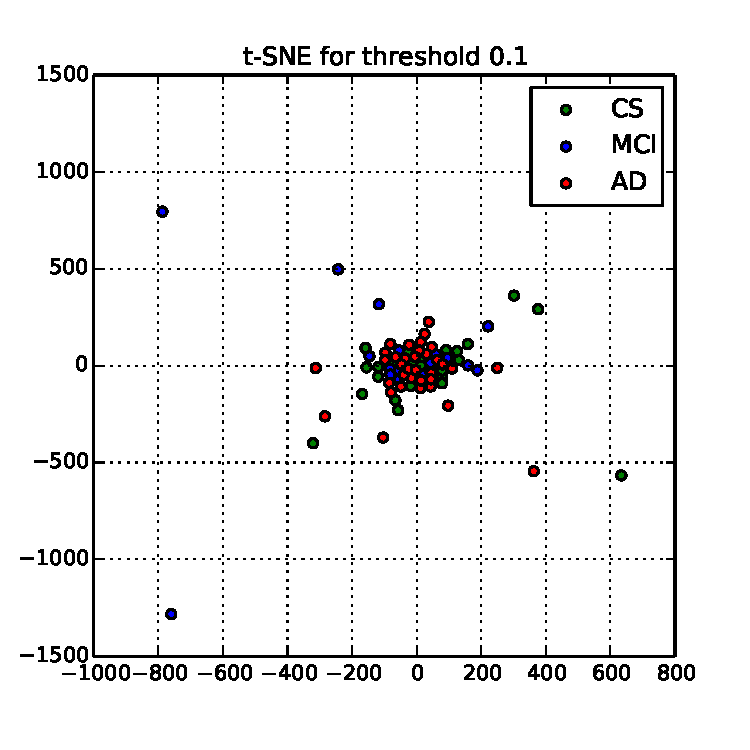
\includegraphics[width=0.7\textwidth]{tSNEThresh2}
		    \caption{t-SNE plot for threshold 0.1.}
		    \label{fig:tsneT2}
		\end{figure}
		\begin{figure}
			\centering
		    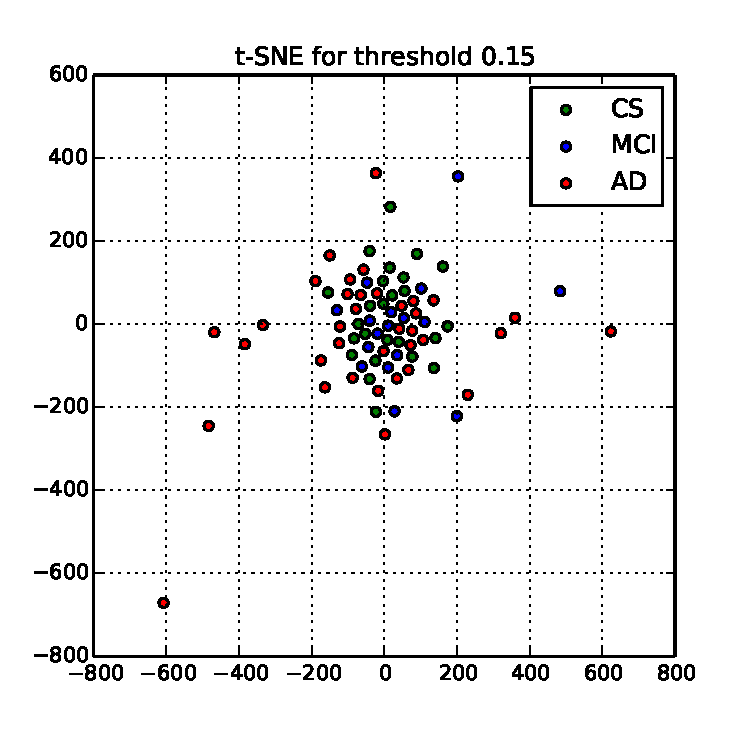
\includegraphics[width=0.7\textwidth]{tSNEThresh3}
		    \caption{t-SNE plot for threshold 0.15.}
		    \label{fig:tsneT3}
		\end{figure}
		\begin{figure}
			\centering
		    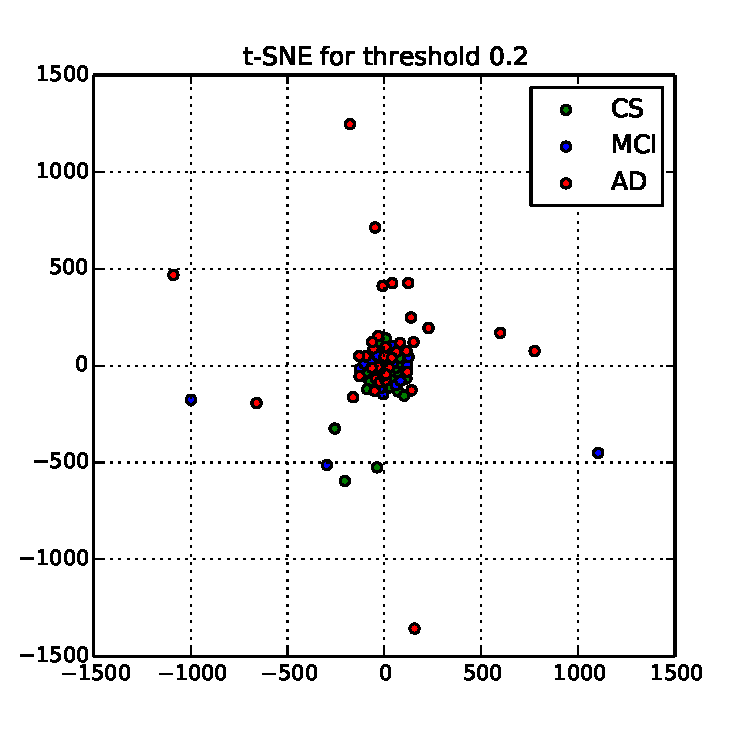
\includegraphics[width=0.7\textwidth]{tSNEThresh4}
		    \caption{t-SNE plot for threshold 0.2.}
		    \label{fig:tsneT4}
		\end{figure}
		\begin{figure}
			\centering
		    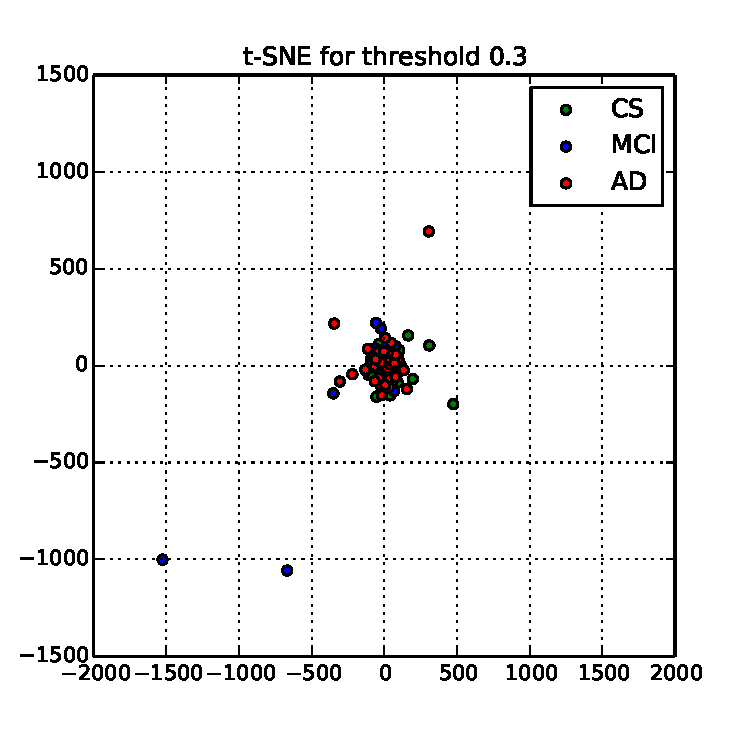
\includegraphics[width=0.7\textwidth]{tSNEThresh5}
		    \caption{t-SNE plot for threshold 0.3.}
		    \label{fig:tsneT5}
		\end{figure}

		\subsection{Box Plots and Parallel Coordinates}
		Box plots can be used to inspect the variance of the graph measures among the subjects. Figure \ref{fig:boxPlot3} shows the box plot of the features computed when looking at the top 15\% strongest links in the connectivity matrices. It can be seen that the most interesting measure is the \ac{SW} value which shows higher variance compared to other measures. Other measures such as \ac{C} and \ac{GE} show large number of outliers which would make it difficult for such metrics to be used for classification. Similar patterns can be seen in the box plots of the other thresholds. These are included in Fig.~\ref{fig:boxPlot1} to \ref{fig:boxPlot5} in Appendix~\ref{appendix:extra-figures}.  

		\begin{figure}
			\centering
		    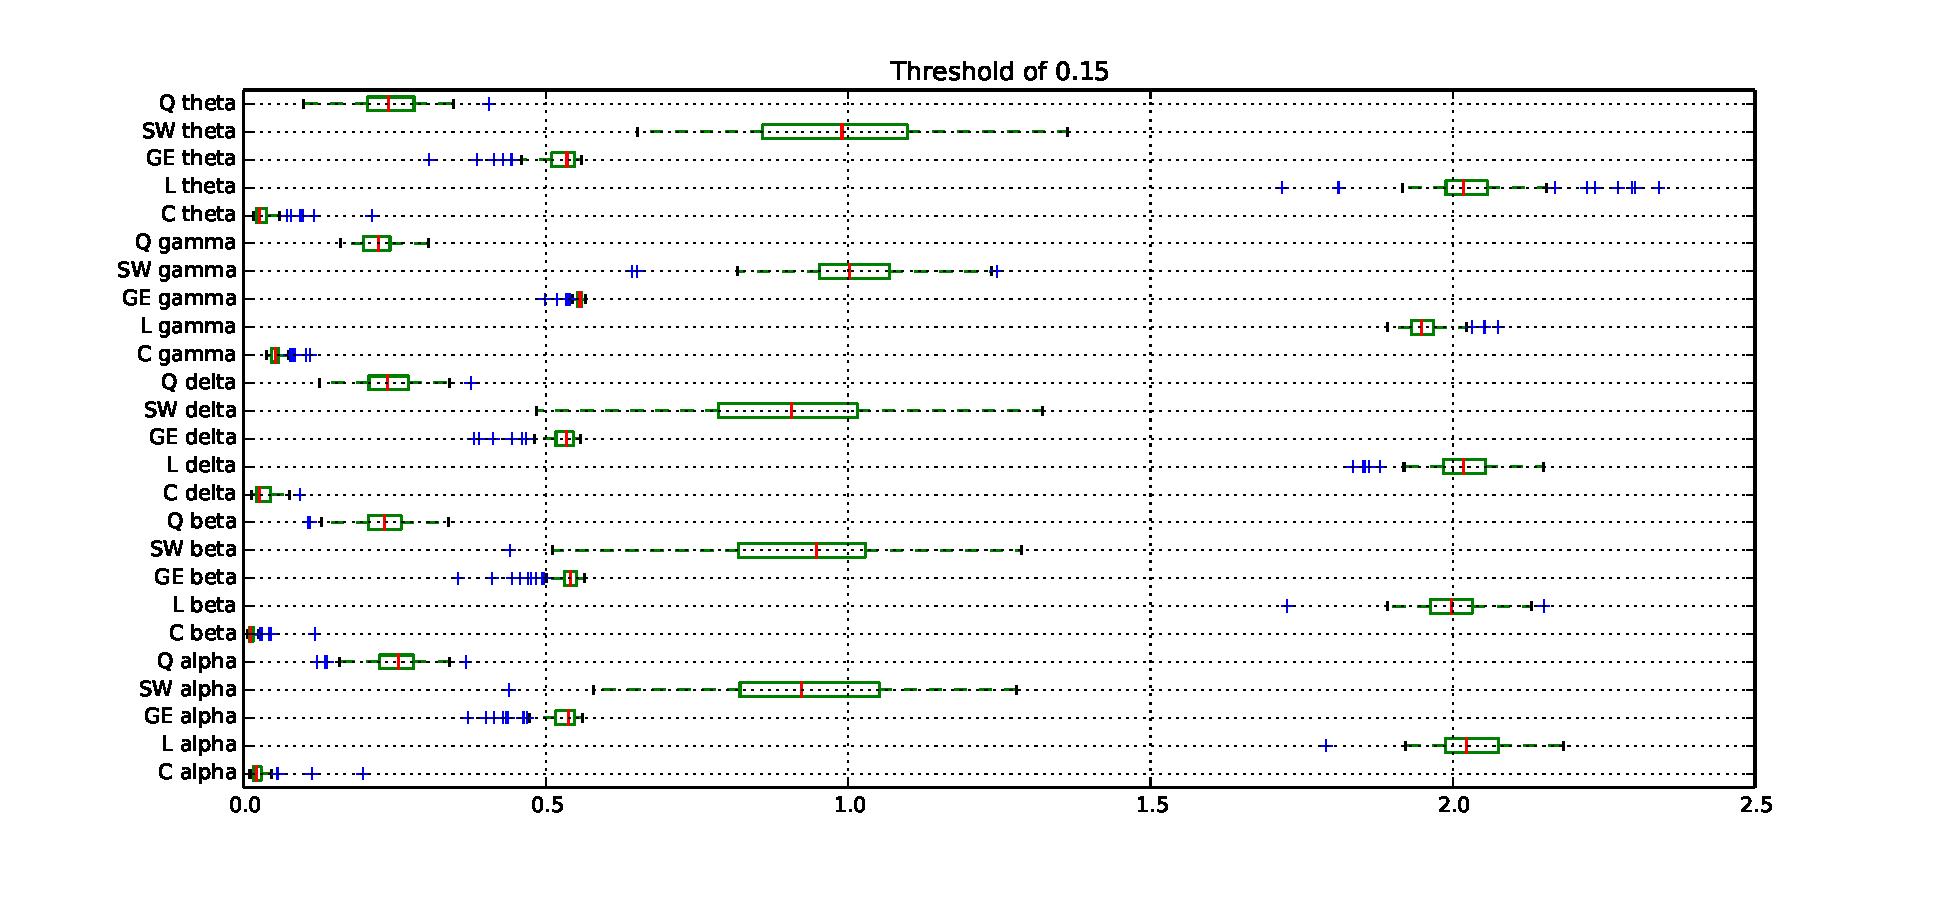
\includegraphics[angle=90, width=0.7\textwidth]{boxplotThresh3}
		    \caption{Box plot of graph measures for threshold 0.15.}
		    \label{fig:boxPlot3}
		\end{figure}
		

		A common way of visualising high-dimensional data is to use parallel coordinates plots. These represent the features of the input data as a set of vertical lines. A data sample is represented as a polyline with vertices on the feature lines. Figure \ref{fig:parallelPlot3} shows a parallel coordinate plot for the features of threshold 0.15. The high overlap of the polylines indicates that there is no clear organisation. The plots for the other thresholds are found in Fig.~\ref{fig:parallelPlot1} to \ref{fig:parallelPlot5} in Appendix~\ref{appendix:extra-figures}.

		\begin{figure}
			\centering
		    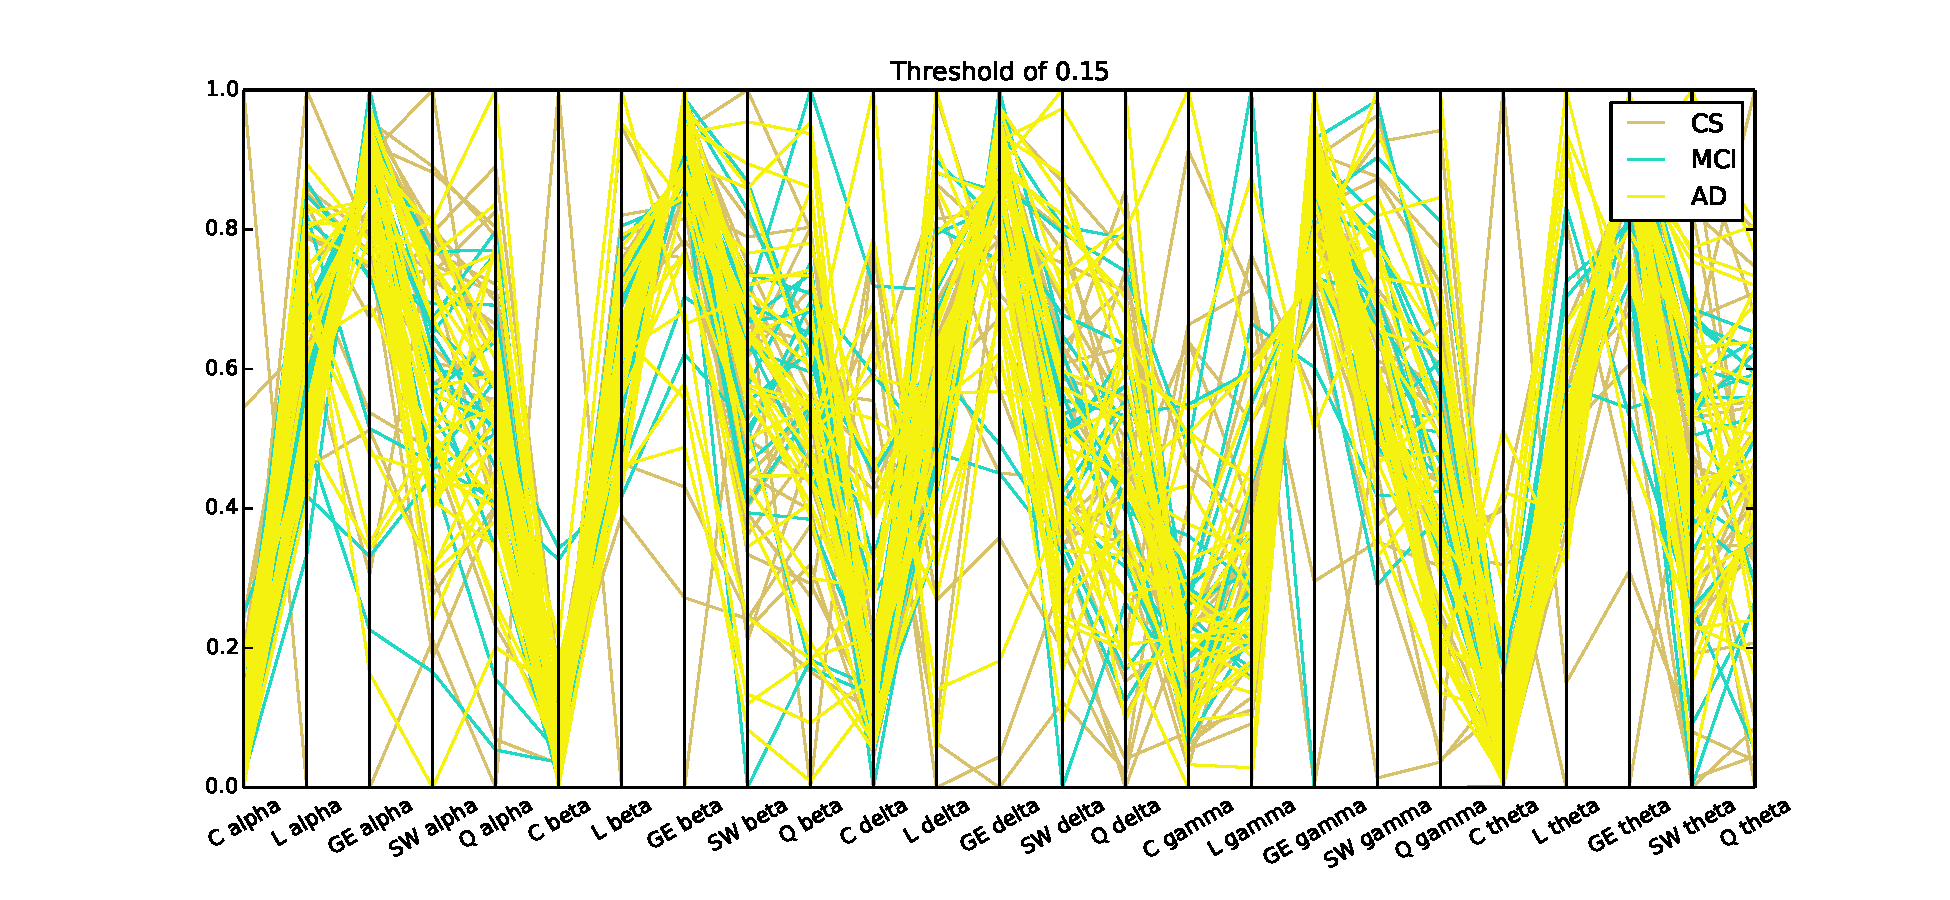
\includegraphics[angle=90, width=0.7\textwidth]{parallelThresh3}
		    \caption{Parallel coordinates plot of graph measures for threshold 0.15.}
		    \label{fig:parallelPlot3}
		\end{figure}


	\section{Classification}
	% confusion matrix and F score
	In this section, the confusion matrices and \(F_1\) scores of the logistic regression and random forest classifier are reported. The classifiers have been trained on the measures from each threshold separately. In addition, classification with just the original data and with the added \ac{SMOTE} samples has been performed.

		\subsection{Confusion Matrices}
				
		The confusion matrices for each algorithm can be found in Appendix~\ref{appendix:confusionmatrices}. A specific matrix can be looked up using Table~\ref{tab:confusion-mats}. 

		\begin{table}
		    \begin{tabular}{|l|l|l|l|l|} \hline
		    Threshold & LR (original)                       & LR (SMOTE)                       & RF (original)                        & RF (SMOTE)                        \\ \hline
		    0.05      & Table \ref{tab:logreg0.05-original} & Table \ref{tab:logreg0.05-smote} & Table \ref{tab:randfor0.05-original} & Table \ref{tab:randfor0.05-smote} \\
		    0.1       & Table \ref{tab:logreg0.1-original}  & Table \ref{tab:logreg0.1-smote}  & Table \ref{tab:randfor0.1-original}  & Table \ref{tab:randfor0.1-smote}  \\
		    0.15      & Table \ref{tab:logreg0.15-original} & Table \ref{tab:logreg0.15-smote} & Table \ref{tab:randfor0.15-original} & Table \ref{tab:randfor0.15-smote} \\
		    0.2       & Table \ref{tab:logreg0.2-original}  & Table \ref{tab:logreg0.2-smote}  & Table \ref{tab:randfor0.2-original}  & Table \ref{tab:randfor0.2-smote}   \\
		    0.3       & Table \ref{tab:logreg0.3-original}  & Table \ref{tab:logreg0.3-smote}  & Table \ref{tab:randfor0.3-original}  & Table \ref{tab:randfor0.3-smote}  \\
		    \hline
		    \end{tabular}
		    \caption{Confusion matrices lookup table. T is the threshold, LR stands for logistic regression and RF is random forest.}
		    \label{tab:confusion-mats}
		\end{table}



		\subsection{\(F_1\) Scores}
		
		Table~\ref{tab:fscores} lists the \(F_1\) scores obtained for the two chosen classifiers.

		\begin{table}
		\centering
		    \begin{tabular}{|l|l|l|l|l|} \hline
		    T & LR (original) & LR (SMOTE) & RF (original) & RF (SMOTE) \\ \hline
		    0.05      & 0.47               & 0.57                 & 0.46                & 0.69                  \\
		    0.1       & 0.43               & 0.57                 & 0.39                & 0.69                  \\
		    0.15      & 0.41               & 0.44                 & 0.39                & 0.69                  \\
		    0.2       & 0.35               & 0.5                  & 0.35                & 0.67                  \\
		    0.3       & 0.35               & 0.4                  & 0.44                & 0.65                  \\
		    \hline
		    \end{tabular}
		    \caption{\(F_1\) scores. T is the threshold, LR stands for logistic regression and RF is random forest.}
		    \label{tab:fscores}
		\end{table}





\section*{Conclusion}
	This chapter presented the computed graph measures with afferent statistics. Results of classification into the three groups of interest were also showed. The next chapter examines these results with respect to the initial project objectives. 
